\chapter{Алгоритми на графах}
\nopagebreak[4]

\section{Вступ}
\nopagebreak[4]
Знаходження найкоротшого шляху на сьогоднішній день є життєво необхідним завданням і використовується практично скрізь, починаючи від знаходження оптимального маршруту між двома об'єктами на місцевості (наприклад, найкоротший шлях від будинку до університету), в системах автопілота, для знаходження оптимального маршруту при перевезеннях, комутації інформаційного пакету в мережах і т.п.

Найкоротший шлях розглядається за допомогою деякого математичного об'єкта, званого графом. Пошук найкоротшого шляху ведеться між двома заданими вершинами в графі. Результатом є шлях, тобто послідовність вершин і ребер, інцидентних двом сусіднім вершинам, і його довжина.

Розглянемо три найбільш ефективних алгоритму знаходження найкоротшого шляху:

\begin{itemize}
\item алгоритм Дейкстри;
\item алгоритм Флойда;
\item Переборні алгоритми. 
\end{itemize}

Зазначені алгоритми легко виконуються при малій кількості вершин у графі. При збільшенні їх кількості завдання пошуку найкоротшого шляху ускладнюється. 




\section{Ключові терміни}
\nopagebreak[4]
\textbf{Алгоритм Дейкстри} - це алгоритм знаходження найкоротшого шляху від однієї з вершин графа до всіх інших, який працює тільки для графів без ребер негативного ваги.

\textbf{Алгоритм Флойда} - це алгоритм пошуку найкоротшого шляху між будь-якими двома вершинами графа.

\textbf{Хвильовий алгоритм} - це переборний алгоритм, який заснований на пошуку в ширину і складається з двох етапів: поширення хвилі і зворотний хід.

\textbf{Найкоротший шлях} - це шлях в графі, тобто послідовність вершин і ребер, інцидентних двом сусіднім вершинам, і його довжина.

Переборний алгоритм - це алгоритм обходу графа, заснований на послідовному переборі можливих шляхів.



\section{Розширені теоретичні відомості}
\subsection{Алгоритм Дейкстри}
\nopagebreak[4]

Даний алгоритм є алгоритмом на графах, який винайдений нідерландським вченим Е. Дейкстрой в 1959 році. Алгоритм знаходить найкоротший відстань від однієї з вершин графа до всіх інших і працює тільки для графів без ребер негативного ваги.

Кожній вершині приписується вага - це вага шляху від початкової вершини до даної. Також кожна вершина може бути виділена. Якщо вершина виділена, то шлях від неї до початкової вершини найкоротший, якщо ні - то тимчасовий. Обходячи граф, алгоритм вважає для кожної вершини маршрут, і, якщо він виявляється найкоротшим, виділяє вершину. Вагою даної вершини стає вага шляху. Для всіх сусідів даної вершини алгоритм також розраховує вагу, при цьому ні за яких умов не виділяючи їх. Алгоритм закінчує свою роботу, дійшовши до кінцевої вершини, і вагою найкоротшого шляху стає вага кінцевої вершини.

Алгоритм Дейкстри
\begin{enumerate}
\item Всім вершинам, за винятком першої, присвоюється вага рівний нескінченності, а першій вершині - 0.

\item Всі вершини не виділені.

\item Перша вершина оголошується поточної.

\item Вага всіх невиділених вершин перераховується за формулою: вага невиділеної вершини є мінімальне число зі старого ваги даної вершини, суми ваги поточної вершини і ваги ребра, що з'єднує поточну вершину з невиділеної.

\item Серед невиділених вершин шукається вершина з мінімальною вагою. Якщо така не знайдена, тобто вага всіх вершин дорівнює нескінченності, то маршрут не існує. Отже, вихід. Інакше, поточної стає знайдена вершина. Вона ж виділяється.

\item Якщо поточною вершиною виявляється кінцева, то шлях знайдений, і його вага є вага кінцевої вершини.

\item Перехід на крок 4.
\end{enumerate}

У програмній реалізації алгоритму Дейкстри побудуємо безліч S вершин, для яких найкоротші шляхи від початкової вершини вже відомі. На кожному кроці до множини S додається та з решти вершин, відстань до якої від початкової вершини менше, ніж для інших, що залишилися вершин. При цьому будемо використовувати масив D, в який записуються довжини найкоротших шляхів для кожної вершини. Коли безліч S буде містити всі вершини графа, тоді масив D міститиме довжини найкоротших шляхів від початкової вершини до кожної вершини.

Крім зазначених масивів будемо використовувати матрицю довжин C, де елемент C [i, j] - довжина ребра (i, j), якщо ребра немає, то її довжина покладається рівною нескінченності, тобто більше будь фактичної довжини ребер. Фактично матриця C являє собою матрицю суміжності, в якій всі нульові елементи замінені на нескінченність.

Для визначення самого найкоротшого шляху введемо масив P вершин, де P [v] буде містити вершину, безпосередньо попередню вершині v в найкоротшому шляху (рис.~\ref{pic:45.1}).
Демонстрація алгоритмом Дейкстри
\begin{figure}
\caption{Демонстрація алгоритму Дейкстри}\label{pic:45.1}
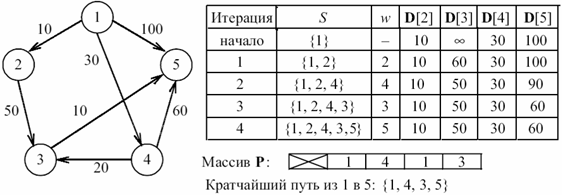
\includegraphics[width=13cm]{pic/45_01.png}

\end{figure}

\begin{lstlisting}[label=code:de,caption=Опис функції алгоритму Дейкстри]
  // Опис функції алгоритму Дейкстри
void Dijkstra (int n, int ** Graph, int Node) {
   bool * S = new bool [n];
   int * D = new int [n];
   int * P = new int [n];
   int i, j;
   int Max_Sum = 0;
   for (i = 0; i <n; i ++)
     for (j = 0; j <n; j ++)
       Max_Sum + = Graph [i] [j];
   for (i = 0; i <n; i ++)
     for (j = 0; j <n; j ++)
       if (Graph [i] [j] == 0) 
         Graph [i] [j] = Max_Sum;
   for (i = 0; i <n; i ++) {
     S [i] = false;
     P [i] = Node;
     D [i] = Graph [Node] [i];
   }
   S [Node] = true;
   P [Node] = -1;
   for (i = 0; i <n - 1; i ++) {
     int w = 0;
     for (j = 1; j <n; j ++) {
       if (! S [w]) {
         if (! S [j] && D [j] <= D [w])
           w = j;
       }
       else w ++;
     }
     S [w] = true;
     for (j = 1; j <n; j ++)
       if (! S [j])
         if (D [w] + Graph [w] [j] <D [j]) {
           D [j] = D [w] + Graph [w] [j];
           P [j] = w;
         }
   }
   for (i = 0; i <n; i ++)
     printf ("% 5d", D [i]);
   cout << endl;
   for (i = 0; i <n; i ++)
     printf ("% 5d", P [i] +1);
   cout << endl;
   delete [] P;
   delete [] D;
   delete [] S;
 } 
\end{lstlisting}

Складність алгоритму Дейкстри залежить від способу знаходження вершини, а також способу зберігання безлічі невідвіданих вершин і способи оновлення довжин.

Якщо для представлення графа використовувати матрицю суміжності, то час виконання цього алгоритму має порядок O (n 2), де n - кількість вершин графа. 

\subsection{Алгоритм Флойда}
Розглянутий алгоритм іноді називають алгоритмом Флойда -Уоршелла. Алгоритм Флойда -Уоршелла є алгоритмом на графах, який розроблений в 1962 році Робертом Флойдом і Стівеном Уоршеллом. Він служить для знаходження найкоротших шляхів між усіма парами вершин графа.

Метод Флойда безпосередньо грунтується на тому факті, що в графі з позитивними вагами ребер всякий Неелементарні (що містить більше 1 ребра) найкоротший шлях складається з інших найкоротших шляхів.

Цей алгоритм більш загальний порівняно з алгоритмом Дейкстри, оскільки він знаходить найкоротші шляхи між будь-якими двома вершинами графа.

В алгоритмі Флойда використовується матриця A розміром nxn, в якій обчислюються довжини найкоротших шляхів. Елемент A [i, j] дорівнює відстані від вершини i до вершини j, яке має кінцеве значення, якщо існує ребро (i, j), і дорівнює нескінченності в іншому випадку.

Алгоритм Флойда

Основна ідея алгоритму. Нехай є три вершини i, j, k і задані відстані між ними. Якщо виконується нерівність $A_{[i, k]} + A_{[k, j]} < A_{[i, j]}$, то доцільно замінити шлях i-> j шляхом i-> k-> j. Така заміна виконується систематично в процесі виконання даного алгоритму.

Крок 0. Визначаємо початкову матрицю відстані A 0 і матрицю послідовності вершин S 0. Кожен діагональний елемент обох матриць дорівнює 0, таким чином, показуючи, що ці елементи в обчисленнях не беруть участь. Вважаємо k = 1.

Основний крок k. Задаємо рядок k і стовпець k як провідну рядок і провідний стовпець. Розглядаємо можливість застосування заміни описаної вище, до всіх елементів A [i, j] матриці A k-1. Якщо виконується нерівність A [i, k] + A [k, j] <A [i, j], (i \ ne k, j \ ne k, i \ ne j) , Тоді виконуємо наступні дії:

    створюємо матрицю A k шляхом заміни в матриці A k-1 елемента A [i, j] на суму A [i, k] + A [k, j];
    створюємо матрицю S k шляхом заміни в матриці S k-1 елемента S [i, j] на k. Вважаємо k = k + 1 і повторюємо крок k. 

Таким чином, алгоритм Флойда робить n ітерацій, після i -й ітерації матриця А буде містити довжини найкоротших шляхів між будь-якими двома парами вершин за умови, що ці шляхи проходять через вершини від першої до i -й. На кожній ітерації перебираються всі пари вершин і шлях між ними скорочується за допомогою i -й вершини (рис.~\ref{pic:45.2}).
Демонстрація алгоритму Флойда
\begin{figure}
\caption{Демонстрація алгоритму Флойда}\label{pic:45.2}
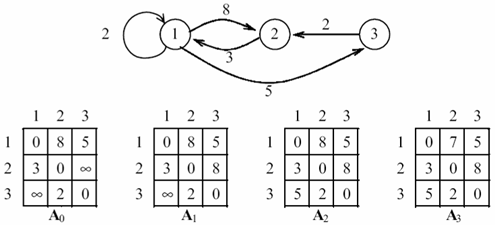
\includegraphics[width=13cm]{pic/45_02.png}

\end{figure}

\begin{lstlisting}[label=code:fl,caption=Опис функції алгоритму Флойда]
  // Опис функції алгоритму Флойда
 void Floyd (int n, int ** Graph, int ** ShortestPath) {
   int i, j, k;
   int Max_Sum = 0;
   for (i = 0; i <n; i ++)
     for (j = 0; j <n; j ++)
       Max_Sum + = ShortestPath [i] [j];
   for (i = 0; i <n; i ++)
     for (j = 0; j <n; j ++)
       if (ShortestPath [i] [j] == 0 && i! = j) 
         ShortestPath [i] [j] = Max_Sum;
   for (k = 0; k <n; k ++)
     for (i = 0; i <n; i ++)
       for (j = 0; j <n; j ++)
         if ((ShortestPath [i] [k] + ShortestPath [k] [j]) < 
              ShortestPath [i] [j])
           ShortestPath [i] [j] = ShortestPath [i] [k] + 
             ShortestPath [k] [j];
 } 
\end{lstlisting}
Зауважимо, що якщо граф неорієнтовний, то всі матриці, одержувані в результаті перетворень симетричні і, отже, досить вираховуватимуть тільки елементи, розташовані вище головної діагоналі.

Якщо граф представлений матрицею суміжності, то час виконання цього алгоритму має порядок O (n 3), оскільки в ньому присутні вкладені одна в одного три циклу. 


\subsection{Переборні алгоритми}

Переборні алгоритми по суті своїй є алгоритмами пошуку, як правило, пошуку оптимального рішення. При цьому рішення конструюється поступово. У цьому випадку зазвичай говорять про перебір вершин дерева варіантів. Вершинами такого графа будуть проміжні або кінцеві варіанти, а ребра вказуватимуть шляху конструювання варіантів.

Розглянемо Переборні алгоритми, засновані на методах пошуку в графі, на прикладі задачі знаходження найкоротшого шляху в лабіринті.

Постановка завдання.

Лабіринт, що складається з прохідних і непрохідних клітин, заданий матрицею A розміром mxn. Елемент матриці A [i, j] = 0, якщо клітина (i, j) прохідна. В іншому випадку $A_{[i, j]} = \infty $.

Потрібно знайти довжину найкоротшого шляху з клітини (1, 1) в клітину (m, n).

Фактично дана матриця суміжності (тільки в ній нулі замінені нескінченності, а одиниці - нулями). Лабіринт являє собою граф.

Вершинами дерева варіантів в даній задачі є шляхи, що починаються в клітці (1, 1). Ребра - показують хід конструювання цих шляхів і з'єднують два шляхи довжини k і k + 1, де другий шлях виходить з першого додаванням до шляху ще одного ходу.

Перебір з поверненням

Даний метод заснований на методі пошуку в глибину. Перебір з поверненням вважають методом проб і помилок ("спробуємо сходити в цю сторону: не вийде - повернемося і спробуємо в іншу"). Так як перебір варіантів здійснюється методом пошуку в глибину, то доцільно під час роботи алгоритму зберігати поточний шлях в дереві. Цей шлях являє собою стек Way.

Також необхідний масив Dist, розмірність якого відповідає кількості вершин графа, який зберігає для кожної вершини відстань від неї до вихідної вершини.

Нехай поточної є деяка клітина (на початку роботи алгоритму - клітина (1, 1)). Якщо для поточної клітини є клітина-сусід Neighbor, відсутня в Way, в яку на цьому шляху ще не ходили, то додаємо Neighbor в Way і поточної клітці присвоюємо Neighbor, інакше витягти з Way.

Наведене вище опис дає чітко зрозуміти, чому цей метод називається перебором з поверненням. Поверненню тут відповідає операція "витягти з Way", яка зменшує довжину Way на 1.

Перебір закінчується, коли Way порожній і робиться спроба повернення назад. У цій ситуації повертатися вже нікуди (рис.~\ref{pic:45.3}).

Way є поточним шляхом, але в процесі роботи необхідно зберігати і оптимальний шлях OptimalWay.

Удосконалення алгоритму можна зробити наступним чином: не дозволяти, щоб довжина Way була більше або дорівнює довжині OptimalWay. У цьому випадку, якщо і буде знайдений якийсь варіант, він свідомо не буде оптимальним. Таке удосконалення в загальному випадку означає, що як тільки поточний шлях стане свідомо неоптимальним, треба повернутися назад. Дане поліпшення алгоритму дозволяє в багатьох випадках сильно скоротити перебір.
Демонстрація алгоритму перебору з поверненням

\begin{figure}
\caption{Демонстрація алгоритму перебору з поверненням}\label{pic:45.3}
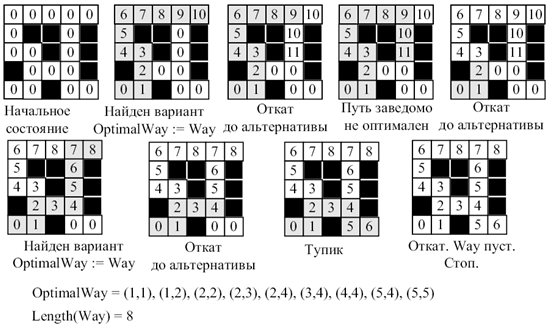
\includegraphics[width=13cm]{pic/45_03.png}
\end{figure}
\begin{lstlisting}
[label=code:pe,caption=Опис функції переборного алгоритму методом пошуку в глибину]
 / * Опис функції переборного алгоритму методом пошуку в глибину * /
void Backtracking (int n, int m, int ** Maze) {
  int Begin, End, Current;
  Begin = (n - 1) * m;
  End = m - 1;
  int * Way, * OptimalWay;
  int LengthWay, LengthOptimalWay;
  Way = new int [n * m];
  OptimalWay = new int [n * m];
  LengthWay = 0;
  LengthOptimalWay = m * n;
  for (int i = 0; i <n * m; i ++)
    Way [i] = OptimalWay [i] = -1;
  int * Dist;
  Dist = new int [n * m];
  for (int i = 0; i <n; i ++)
    for (int j = 0; j <m; j ++)
      Dist [i * m + j] = (Maze [i] [j] == 0? 0: -1);
  Way [LengthWay ++] = Current = Begin;
  while (LengthWay> 0) {
    if (Current == End) {
      if (LengthWay <LengthOptimalWay) {
        for (int i = 0; i <LengthWay; i ++)
          OptimalWay [i] = Way [i];
        LengthOptimalWay = LengthWay;
       }
      if (LengthWay> 0) Way [- LengthWay] = -1;
      Current = Way [LengthWay-1];
     }
    else {
      int Neighbor = -1;
      if ((Current / m - 1)> = 0 &&! Insert (Way, Current - m) &&
        (Dist [Current - m] == 0 || Dist [Current - m]> LengthWay)
        && Dist [Current] <LengthOptimalWay)
          Neighbor = Current - m;
       else 
        if ((Current% m - 1)> = 0 &&! Insert (Way, Current - 1) &&
          (Dist [Current - 1] == 0 || Dist [Current - 1]> LengthWay)
          && Dist [Current] <LengthOptimalWay)
            Neighbor = Current - 1;
         else 
          if ((Current% m + 1) <m &&! Insert (Way, Current + 1) &&
           (Dist [Current + 1] == 0 || Dist [Current + 1]> LengthWay)
          && Dist [Current] <LengthOptimalWay)
            Neighbor = Current + 1;
          else 
           if ((Current / m + 1) <n &&! Insert (Way, Current + m) &&
            (Dist [Current + m] == 0 || Dist [Current + m]> LengthWay)
           && Dist [Current] <LengthOptimalWay)
             Neighbor = Current + m;
      if (Neighbor! = -1) {
        Way [LengthWay ++] = Neighbor;
        Dist [Neighbor] = Dist [Current] + 1;
        Current = Neighbor;
       }
       else {
        if (LengthWay> 0) Way [- LengthWay] = -1;
        Current = Way [LengthWay-1];
       }
     }
   }
  if (LengthOptimalWay <n * m) 
    cout << endl << "Yes. Length way =" << LengthOptimalWay << endl;
  else cout << endl << "No" << endl;
 } 
\end{lstlisting}


\subsection{Хвильовий алгоритм}

Цей переборний алгоритм, який заснований на пошуку в ширину, складається з двох етапів:
\begin{itemize}
\item поширення хвилі;
\item зворотний хід.
\end{itemize}
 
Поширення хвилі і є власне пошук в ширину, при якому клітини позначаються номером кроку методу, на якому клітина відвідується. При зворотному ході, починаючи з кінцевої вершини, йде відновлення шляху, по якому в неї потрапили шляхом включення до нього клітин з мінімальною позначкою (рис.~\ref{pic:45.4}). Важливою особливістю є те, що відновлення починається з кінця (з початку воно найчастіше неможливо).
Демонстрація хвильового алгоритму

\begin{figure}
\caption{Демонстрація хвильового алгоритму}\label{pic:45.4}
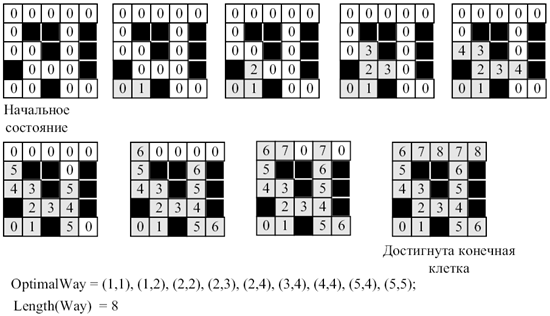
\includegraphics[width=13cm]{pic/45_04.png}
\end{figure}


Зауважимо, що перебір методом пошуку в ширину в порівнянні з перебором з поверненням, як правило, вимагає більше допоміжної пам'яті, яка необхідна для зберігання інформації, щоб побудувати шлях при зворотному ході і помітити відвідані вершини. Однак він працює швидше, оскільки абсолютно виключається відвідування однієї і тієї ж клітини більш ніж один раз.

\section{Приклади обчислень}
\nopagebreak[4]




\subsection*{Контрольні запитання}
\nopagebreak[4]
\begin{enumerate}
\item ?
\end{enumerate}



